\documentclass{beamer}

\usepackage{beamerthemesplit}
\usepackage[utf8]{inputenc}
\usepackage[ngerman]{babel}
\usepackage[justification=centering,figurename=Abb.]{caption}
\usepackage{pdfpages} 
\usepackage{listings} 
\usepackage{color}

\definecolor{dkgreen}{rgb}{0,0.6,0}
\definecolor{gray}{rgb}{0.5,0.5,0.5}
\definecolor{mauve}{rgb}{0.58,0,0.82}

\usetheme{Boadilla}
\useoutertheme[footline=authortitle]{miniframes}
\useinnertheme{rectangles}

\lstset{
    language=Java,
    tabsize=4,
    keepspaces,
    extendedchars=true,
    rulecolor=\color{black},
    keywordstyle=\color{blue},
    commentstyle=\color{dkgreen},
    stringstyle=\color{mauve},
    basicstyle=\footnotesize,
    aboveskip=5pt,
    upquote=true,
    columns=fixed,
    showstringspaces=false,
    extendedchars=true,
    breaklines=true,
    frame=single,
    showtabs=true,
    showspaces=false,
    showstringspaces=false,
}

\beamertemplatenavigationsymbolsempty

\title{Vortrag III: Abschluss Entwicklung einer GUI für den gMix-Simulator} 
\author[M. Weinschenk, J. Langnickel, J.C. Lohmüller, A. Beifuß]{Malte Weinschenk, Jörg Langnickel, \\ Jan Carsten Lohmüller \& Alexander Beifuß} 
\date{\today} 


\begin{document}

\frame{\titlepage} 

\frame[t,squeeze]{\frametitle{Inhalt}
	\tableofcontents
}

\section[Einleitung]{Einleitung}
\frame[t,squeeze]{\frametitle{Ausgangssituation gMix}
   \begin{itemize}
		\item Last Generierung
			\begin{itemize}
				\item Bestimmung von Lastcharakteristika
				\item Modellierung der Clients
			\end{itemize}
		\item Simulation \& Messung
			\begin{itemize}
				\item Modellierung  der Mixe
				\item Konfiguration der Plug-Ins
			\end{itemize}
		\item Evaluation
			\begin{itemize}
				\item Auswertungs Plug-Ins
			\end{itemize}
	\end{itemize}
	
}

\frame[t,squeeze]{\frametitle{Motivation}
   
}

\frame[t,squeeze]{\frametitle{Benutzergruppen}
   \begin{block}{}
    \begin{enumerate}
        \item<+-> Nutzer in der Lehre
            \begin{itemize}
                \item Das System muss einfach zu bedienen sein
                \item Vermeidung einer überladenen GUI mit zu viel Details
                \item Unterstützung durch die GUI bei der Fehlervermeidung
                \item Übersichtliche Präsentation der Ergebnisse
            \end{itemize}
        \item<+-> Nutzer in der Forschung
            \begin{itemize}
                \item Kontrolle über viele / alle Parameter
                \item Flexible Darstellung der Ergebnisse
                \item Stapelverarbeitung von Experimenten
            \end{itemize}
        \item<+-> Plug-In Entwickler
            \begin{itemize}
                \item Möglichst wenig Aufwand bei der GUI
                \item Plug-in soll entkoppelt betrachtet werden
                \item Es sollen keine Namenskollisionen mit anderen Plug-ins entstehen
            \end{itemize}
    \end{enumerate}
    \end{block}
}

\frame[t,squeeze]{\frametitle{Ziele}
   \begin{block}{Projektziel:}
    \begin{enumerate}
        \item Grafisches Werkzeug zur Erstellung von gMix-Konfigurationen
        \item Augenmerk auf Anwenderfreundlichkeit
        \item Augenmerk auf Entwicklerfreundlichkeit
    \end{enumerate}
  \end{block}  
}

\section[GUI]{GUI}

\frame[t,squeeze]{\frametitle{Designidee}
   \begin{figure}
        \centering
        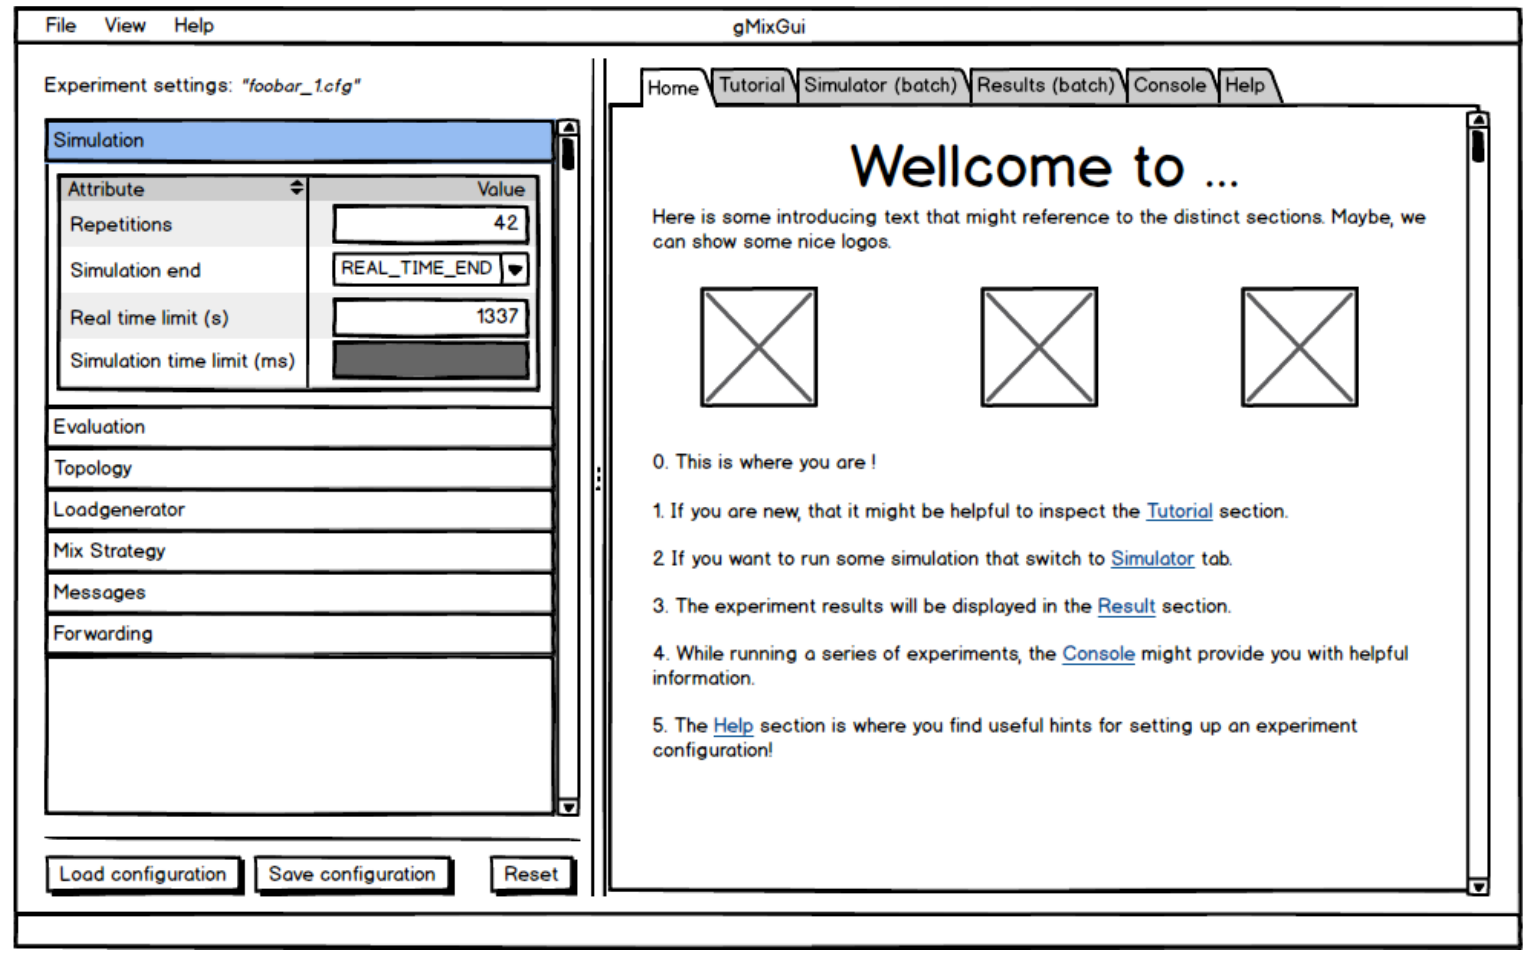
\includegraphics[scale=0.20]{simgui_mockup.png}
    \end{figure}
}

\frame[t,squeeze]{\frametitle{Erste Umsetzung}
   \begin{figure}
        \centering
        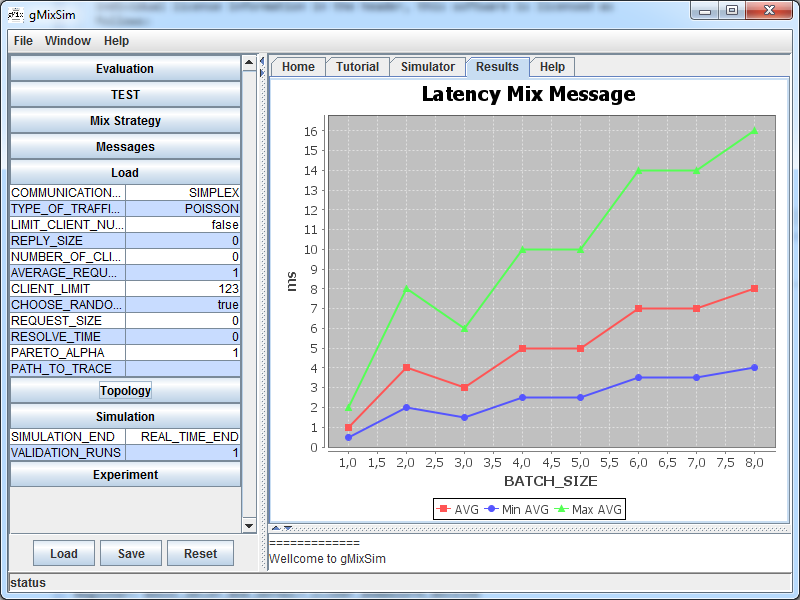
\includegraphics[scale=0.30]{results.png}
    \end{figure}
}

\frame[t,squeeze]{\frametitle{gMixGUI}
   \begin{figure}
        \centering
        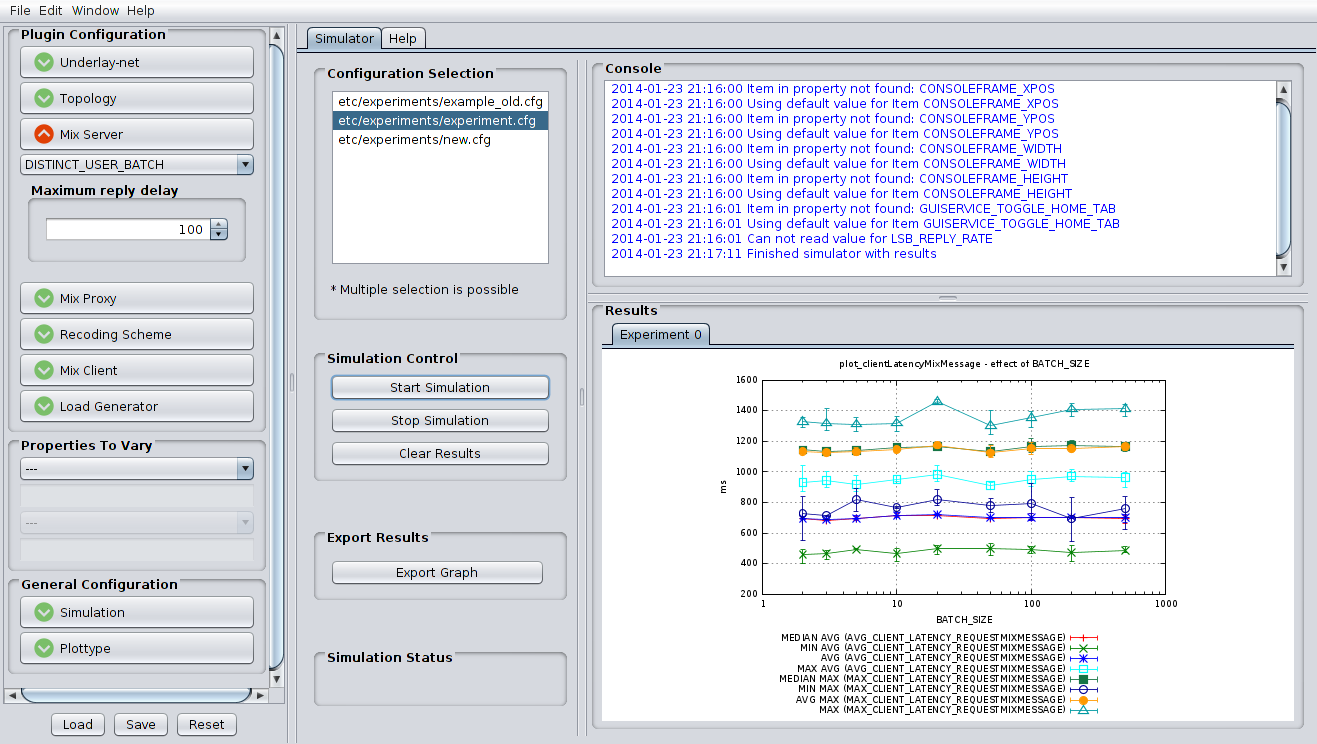
\includegraphics[scale=0.23]{simgui.png}
    \end{figure}
}

\section[Architektur]{Architektur}

\frame[t,squeeze]{\frametitle{Architektur}
   \begin{figure}
        \centering
        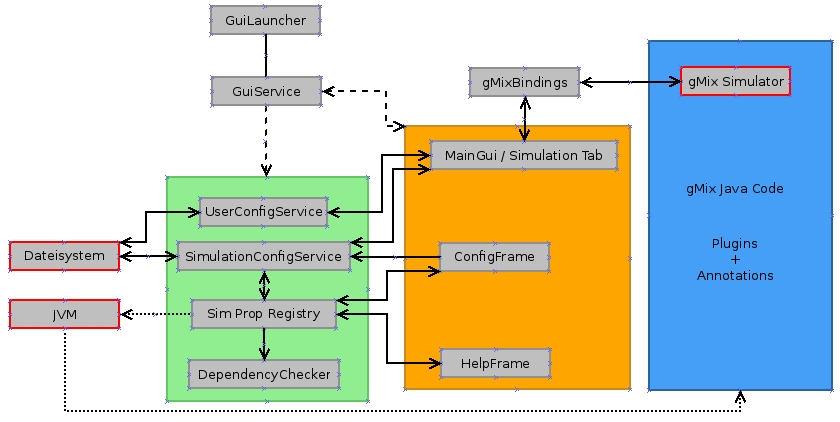
\includegraphics[scale=0.8]{arch.png}
   \end{figure}
}

\section[Annotations]{Annotations}

\frame[t,squeeze]{\frametitle{Motivation für die Verwendung von Annotationen}

\small{
   \begin{tabular}{|l|c|c|c|c|}
   \hline
    & Annotationen & XML zentr. & XML dezentr. & Statisch \\
   \hline\hline
   Plugin Struktur & ++ & - & + & - -\\
   Initialer Aufwand & - & ++ & + & ++ \\
   Aufwand neues Plugin & ++ & + & + & - - \\
   Erweiterbarkeit Fkt. & + & +(+) & +(+) & ? \\
   % Übersichtlichkeit & - & ++ & + & ++ \\
   Unterstützung d. IDE & ++ & + & + & ++ \\
   \hline
   \end{tabular}

}

    \begin{block}{}
    Für GUI-Benutzer ist die verwendete Technik transparent.\\
    Plugin-Entwickler profitieren jedoch sehr von den Annotations.\\
    $\Rightarrow$ Es sind wenig Gedanken zur GUI nötig.\\
    $\Rightarrow$ Rapid Prototyping\\
    Der Mehraufwand bei der Programmierung des Frameworks ist gerechtfertigt.
    \end{block}
}

\begin{frame}[fragile]{Anwendungsbeispiel für Annotationen}
    \begin{lstlisting}
@PluginSuperclass(
    layerName = "Underlay-net",
    layerKey = "TYPE_OF_DELAY_BOX",
    position = 7)
public abstract class DelayBoxImpl {
    \end{lstlisting}
    \begin{lstlisting}
@Plugin(
    pluginName = "Basic delay",
    pluginKey = "BASIC_DELAY_BOX")
public class BasicDelayBox extends DelayBoxImpl {

    @IntSimulationProperty(
        name = "Packet Size (byte)",
        key = "NETWORK_PACKET_PAYLOAD_SIZE")
    private int packetSize = new ...
    \end{lstlisting}
\end{frame}

% \frame[t,squeeze]{\frametitle{Aenderungen an der EDF\_VERSION notwendig}

%     \begin{block}{EDF\_VERSION (Experiment Definition File)}
%     \begin{itemize}
%         \item Property- und Pluginkeys müssen eindeutig sein\\
%         BATCH\_SIZE ( BASIC\_BATCH / BATCH\_WITH\_TIMEOUT )\\
%         NO\_DELAY ( OUTPUT\_STRATEGY / TYPE\_OF\_DELAY\_BOX )\\
%         \item Einführung von EDF\_VERSION\_1 für die GUI
%         \item Nicht kompatibel zu EDF\_VERSION\_0
%     \end{itemize}
%     \end{block}
% }

\section[Dependency Checker]{Dependency Checker}

\frame[t,squeeze]{\frametitle{Dependency Checker}
\begin{itemize}
		\item Konfigurationsdateien
		\item Keine Unterstützung von Abhängigkeiten und Wertebereichen
		\item Abhängigkeiten zwischen Properties: 
					\begin{itemize}
					\item Value Requirements z.B. Minimal- und Maximalwerte
					\item Enable Requirements z.B. gegenseitiger Ausschluß
				\end{itemize}
		\item Wertebereiche in einem Property: Minimal- und Maximalwerte
		\item Ziele:
					\begin{itemize}
					\item Einfache Benutzung
					\item Maximale Flexibilität
					\item Wertebereiche in einem Property beachten
				\end{itemize}
\end{itemize}
   
}

\section[Live Demo]{Live Demo}

\frame[t,squeeze]{\frametitle{Live Demo}
   \vspace{3em}
   \centering{\large{Live Demo}}
}

\section*{Ende}

\frame[t,squeeze]{\frametitle{Ende}
   \vspace{3em}
   \centering{\large{Vielen Dank für Ihre Aufmerksamkeit}}
}

% \frame[t,squeeze]{\frametitle{Nutzergruppen}
% 	\begin{block}{}
%     \begin{enumerate}
%         \item<+-> Nutzer in der Lehre
%             \begin{itemize}
%                 \item Das System muss einfach zu bedienen sein
%                 \item Vermeidung einer überladenen GUI mit zu viel Details
%                 \item Unterstützung durch die GUI bei der Fehlervermeidung
%                 \item Übersichtliche Präsentation der Ergebnisse
%             \end{itemize}
%         \item<+-> Nutzer in der Forschung
%             \begin{itemize}
%                 \item Kontrolle über viele / alle Parameter
%                 \item Flexible Darstellung der Ergebnisse
%                 \item Stapelverarbeitung von Experimenten
%             \end{itemize}
%         \item<+-> Plug-In Entwickler
%             \begin{itemize}
%                 \item Möglichst wenig Aufwand bei der GUI
%                 \item Plug-in soll entkoppelt betrachtet werden
%                 \item Es sollen keine Namenskollisionen mit anderen Plug-ins entstehen
%             \end{itemize}
%     \end{enumerate}
%     \end{block}
% }

% \section[Letzter Entwicklungsstand]{Letzter Entwicklungsstand}

% \frame[t,squeeze]{\frametitle{Willkommens Reiter}
%     \begin{figure}
%         \centering
%         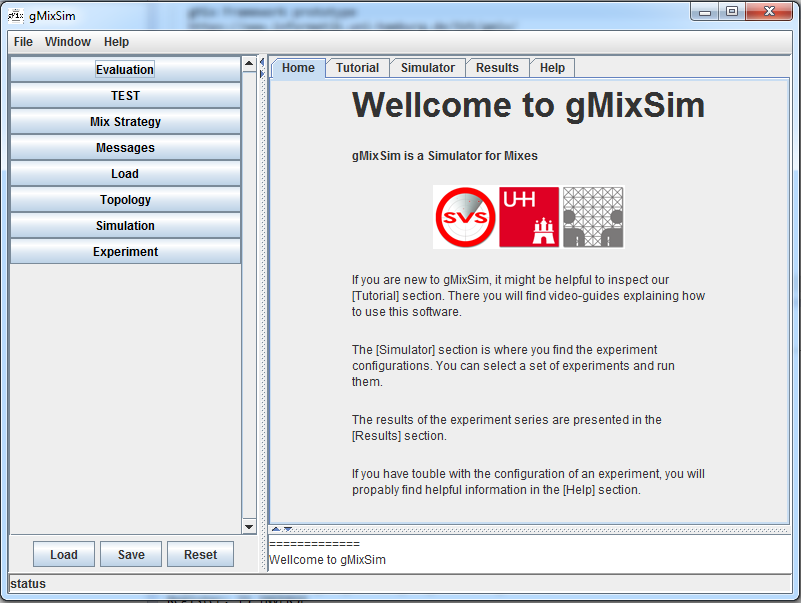
\includegraphics[scale=0.32]{wellcome.png}
%     \end{figure}
% }

% \frame[t,squeeze]{\frametitle{Tutorial Reiter}
%     \begin{figure}
%         \centering
%         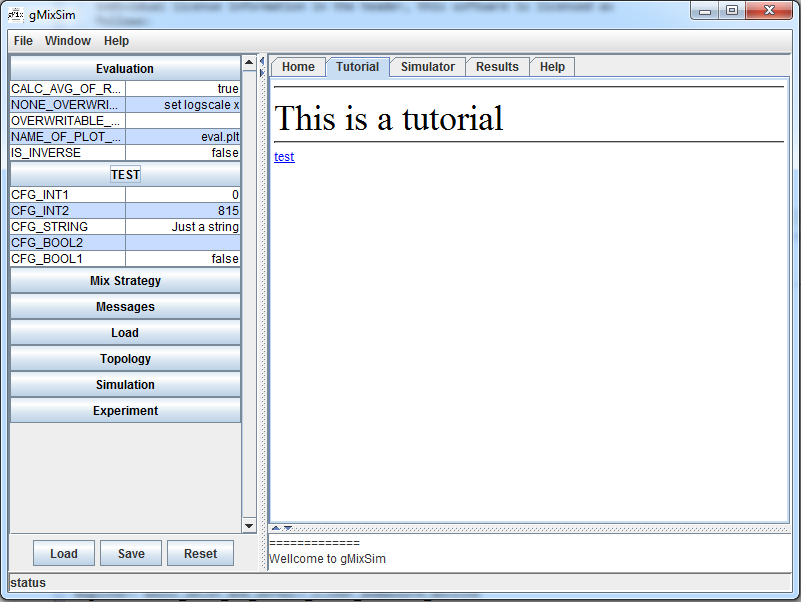
\includegraphics[scale=0.32]{tutorial.png}
%     \end{figure}
% }

% \frame[t,squeeze]{\frametitle{Simulator Reiter}
%     \begin{figure}
%         \centering
%         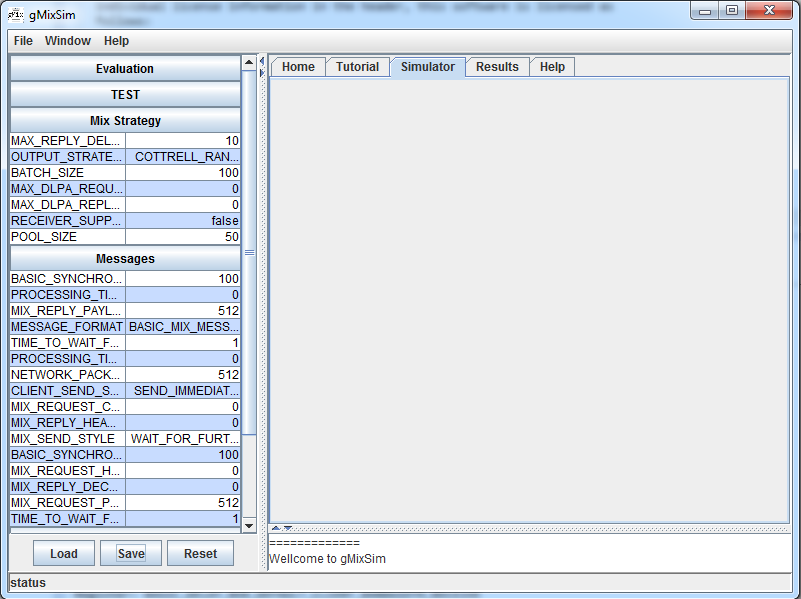
\includegraphics[scale=0.32]{simwindow.png}
%     \end{figure}
% }

% \frame[t,squeeze]{\frametitle{Ergebnis Reiter}
%     \begin{figure}
%         \centering
%         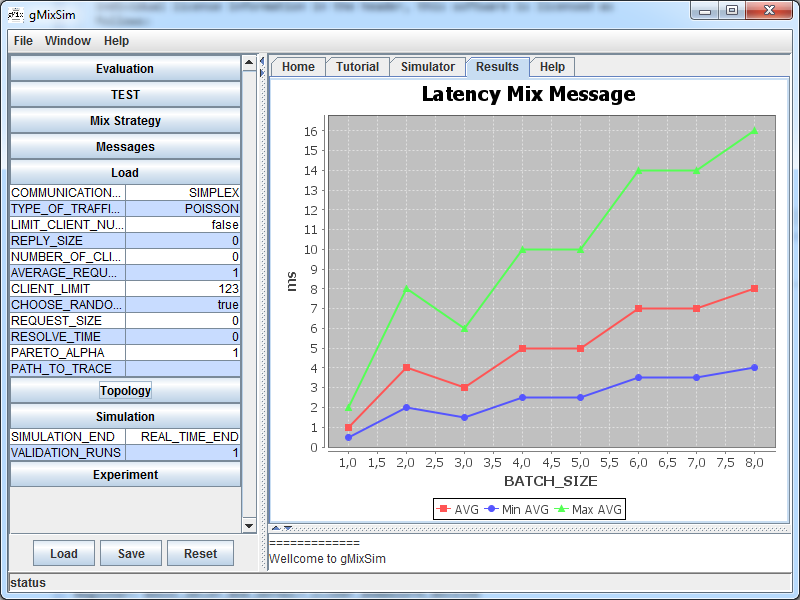
\includegraphics[scale=0.32]{results.png}
%     \end{figure}
% }

% \frame[t,squeeze]{\frametitle{Hilfe Reiter}
%     \begin{figure}
%         \centering
%         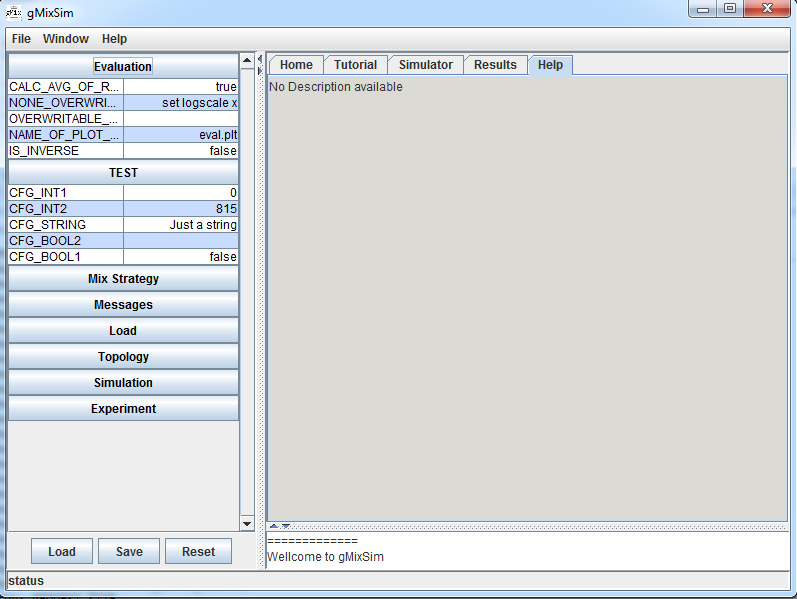
\includegraphics[scale=0.32]{menu.png}
%     \end{figure}
% }

% \frame[t,squeeze]{\frametitle{Aufgaben}
%     \begin{block}{Hauptkritikpunkte aus der letzten Besprechung}
%         \begin{enumerate}
%             \item Fenster (Hilfe und Konfigurationswerkzeug) entkoppelbar machen
%             \item Hilfe und Tutorial in eins zusammenfassen
%             \item Simulator- und Ergebnis-Tabs zusammenfassen
%             \item Visuelle Unterstützung der Accordion-Elemente durch Icons
%         \end{enumerate}
%     \end{block}
% }

% \section[Aktueller Entwicklungsstand (live demo)]{Aktueller Entwicklungsstand (Live Demo)}

% \frame[t,squeeze]{\frametitle{Fortschritt}
%     \begin{block}{Implementiert}
%         \begin{enumerate}
%             \item Hilfe- und Konfigurationsfenster entkoppelbar
%             \item Hilfe und Tutorial zusammengefasst (basieren auf HTML)
%             \item Benutzer Konfigurationen bzgl. GUI können gespeichert werden
%             \item Abhängigkeiten zwischen Konfigurations-Attributen können festgelegt werden
%             \item Problematische Werte werden durch Fehlermeldung aufgezeigt
%             \item Plug-Ins können anhand des Classpaths eingelesen werden
%             \item Typspezifische Annotations für String, Bool, Int und Float
%             \item Simulator ist aus der GUI aufrufbar
%             \item Visuelle Unterstützung der Accordion-Elemente durch Icons
%         \end{enumerate}
%     \end{block}
% }

% \frame{\frametitle{}
%     \centering
%     \fontsize{32pt}{7.2}\selectfont{Live Demonstration}
% }


% \section[Ausblick auf geplante Features]{Ausblick auf geplante Features}

% \frame[t,squeeze]{\frametitle{Ausblick auf geplante Features I}
% 	\begin{block}{Quick Wins}
% 		\begin{enumerate}
%             \item Ausblenden des Home-Tabs ermöglichen
% 			\item Laden und Speichern von Konfigurationen
% 				\begin{itemize}
% 					\item Sowie Übergabe der Konfigurationen an den Simulator
% 				\end{itemize}
% 			\item Rendern der Simulationsergebnisse
%                 \begin{itemize}
%                     \item In gesonderten Tabs oder entkoppelten Fenstern
%                 \end{itemize}
% 			\item Annotations auf das gMix-Projekt anwenden
%             \item GUI für den Simulator-Tab
% 		\end{enumerate}
% 	\end{block}
% }

% \frame[t,squeeze]{\frametitle{Ausblick auf geplante Features II}
% 	\begin{block}{Weitere Entwicklung der Annotations}
%         \begin{enumerate}
% 		\item Dependency-Violations
% 			\begin{itemize}
% 				\item Visuelle Unterstützung des Benutzers durch Anzeige von Abhängigkeiten (\texttt{Feature Models})
% 			\end{itemize}
% 		\item Plugin-Annotations
% 			\begin{itemize}
% 				\item Modellierung von Plugin-Abhängigkeiten (Level 1 bis Level 5)
% 			\end{itemize}
% 		\item (Dependency-)Service-Plugin 
% 			\begin{itemize}
% 				\item Ebenfalls Modellierung von Plugin-Abhängigkeiten
% 			\end{itemize}
% 		\item Dynamisches Erstellen der Hilfe basierend auf Annotations
%             \begin{itemize}
%                 \item z.B. Minimum- und Maximumwerte aus den Annotations extrahieren
%             \end{itemize}
% 		\item Grafische Elemente anstatt Attribut-Tabelle
% 			\begin{itemize}
% 				\item z.B. Spinner für Integer, Textbox für freie Strings, Dropdownmenu für vordefinierte Werte
% 			\end{itemize}
% 		\end{enumerate}
% 	\end{block}
% }
% %\begin{frame}[allowframebreaks]
% %\frametitle{Quellen}
% %\nocite{*}
% %\printbibliography
% %\end{frame}

% \section{Diskussion}
% \frame{
% \begin{center}
% 	\huge{Diskussion}
% \end{center}
% }


\end{document}
